\documentclass{article}

\title{Automata and Languages}
\author{Amit Rajaraman}
\date{March 2020}

\usepackage[utf8]{inputenc}
\usepackage{amsmath}
\usepackage{amssymb}
\usepackage{amsthm}
\usepackage{amsfonts}
\usepackage{enumerate}
\usepackage[margin=1in]{geometry}
\usepackage[colorlinks]{hyperref}
\usepackage{tikz}
\usetikzlibrary{automata, positioning, arrows, matrix}
\tikzset{->, >=stealth', node distance = 2cm}

\usepackage{titlesec}
\titleformat{\section}[block]{\sffamily\Large\filcenter\bfseries}{\S\thesection.}{0.25cm}{\Large}
\titleformat{\subsection}[block]{\large\bfseries\sffamily}{\thesubsection.}{0.2cm}{\large}

\usepackage{fancyhdr}
\lhead{\sffamily{Automata and Languages}}
\chead{\sffamily{\thepage}}
\rhead{\sffamily{-Amit Rajaraman}}
\cfoot{}
\pagestyle{fancy}

\setlength\parindent{0pt}

\renewcommand{\qedsymbol}{$\blacksquare$}

\newcommand{\yields}{\Rightarrow}
\newcommand{\derives}{\overset{*}{\yields}}
\newcommand{\writeNPDA}{(Q,\Sigma,\Gamma,\delta,q_0,Z_0,F)}

\numberwithin{equation}{section}
\theoremstyle{definition}
\newtheorem{theorem}{Theorem}
\newtheorem{lemma}[theorem]{Lemma}
\newtheorem{corollary}[theorem]{Corollary}
\newtheorem{definition}{Definition}
\numberwithin{definition}{section}
\numberwithin{theorem}{section}
\newtheorem{exercise}{Exercise}
\newtheorem*{example}{Example}

\theoremstyle{remark}
\numberwithin{exercise}{section}
\newtheorem*{solution}{Solution}

\begin{document}

\maketitle
\thispagestyle{empty}

\tableofcontents
\clearpage

\section{Regular Languages}

Before we proceed any further, a question we must ask is - what \textit{is} a computer? The computers we use are probably too complicated to model as a mathematical system. So we shall try to create an idealized computer called a \textit{computational model}. Like models in general, this model is realistic in some ways, and unrealistic in others.

\subsection{Finite Automata}

Finite automata are a good place to begin that are good models for computers with an extremely limited amount of memory.

\begin{example}
For starters, consider an automatic door controller. It has a front pad, a back pad and a door. The door can be either open or closed and each of the pads can be either pressed or not pressed. Using this, we can construct a ``state diagram'' to show how the state of the system proceeds:
\begin{center}
  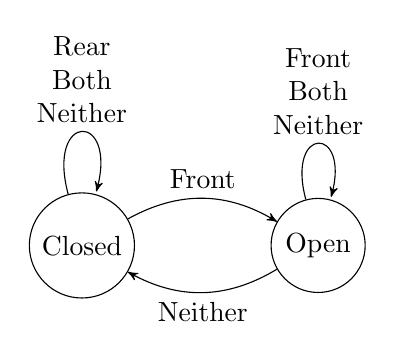
\begin{tikzpicture}[node distance=3cm]
    \node[state] (1) {Closed};
    \node[state] (2) [right of=1] {Open};

    \draw (1) edge[loop above] node[align=center]{Rear\\ Both\\ Neither} (1)
          (2) edge[loop above] node[align=center]{Front\\ Both\\ Neither} (2)
          (1) edge[bend left, above] node{Front} (2)
          (2) edge[bend left, below] node{Neither} (1);
    \end{tikzpicture}
\end{center}

It can also be represented by the following table:
\begin{center}
\begin{tabular}{l|llll}
       & Front  & Back   & Neither & Both   \\ \hline
Closed & Open   & Closed & Closed  & Closed \\
Open   & Closed & Closed & Open    & Closed  
\end{tabular}
\end{center}
\end{example}
~\\
Thinking of a finite automaton like this automatic door controller, which has only a single bit of memory, suggests standard ways to represent automata as a state transition graph or a  state transition table.

Finite automata, and their probabilistic counterparts, \textit{Markov Chains}, are very useful tools.

Let us look at another finite automaton to cement the idea before exactly defining what it is.

\begin{example}
Consider the following state diagram of an automaton $M$.
\begin{center}
  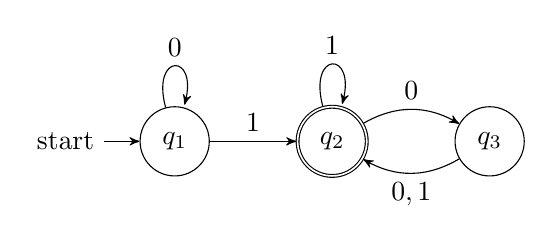
\begin{tikzpicture}
    \node[state, initial] (q1) {$q_1$};
    \node[state, accepting, right of=q1] (q2) {$q_2$};
    \node[state, right of=q2] (q3) {$q_3$};
    \draw (q1) edge[loop above] node{$0$} (q1)
          (q2) edge[loop above] node{$1$} (q2)
          (q1) edge[above] node{$1$} (q2)
          (q2) edge[bend left, above] node{$0$} (q3)
          (q3) edge[bend left, below] node{$0,1$} (q2);
    \end{tikzpicture}
\end{center}
It has three ``states'', $q_1, q_2$ and $q_3$. The \textit{start state}, $q_1$ is indicated as shown. The \textit{accept state}, $q_2$ is indicated by the double circle. The arrows are called \textit{transitions}. When the automaton receives some input string like \texttt{11001}, it processes the string and produces some output, \textit{accept} or \textit{reject}. For now, we will consider only yes/no questions like this one.

An already obvious question to ask is that what language of input strings give an accept output? We will answer this soon.
\end{example}

\begin{definition}
A \textit{deterministic finite automaton} is a $5$-tuple $(Q,\Sigma, \delta, q_0, F)$ where
\begin{itemize}
    \item $Q$ is a finite set called the set of \textit{states}.
    \item $\Sigma$ is a finite set of input symbols called the \textit{alphabet}.
    \item $\delta:Q\times\Sigma\to Q$ is the \textit{transition function}.
    \item $q_0\in Q$ is the \textit{start state}.
    \item $F\subseteq Q$ is the \textit{set of accept states}.
\end{itemize}
\end{definition}

Accept states are also sometimes called \textit{final states}.

\begin{example}
The finite automaton $M$ we described earlier can be put in this format in the following way: 
\begin{itemize}
    \item $Q=\{q_1,q_2,q_3\}$
    \item $\Sigma=\{0,1\}$
    \item $\delta$ is described as follows:
    \begin{center}
        \begin{tabular}{l|ll}
            & $0$  & $1$   \\ \hline
            $q_1$ & $q_1$   & $q_2$\\
            $q_2$ & $q_3$ & $q_2$\\
            $q_3$ & $q_2$ & $q_2$
        \end{tabular}
    \end{center}
    \item $q_1$ is the start state, and
    \item $F=\{q_2\}$
\end{itemize}
\end{example}

If $A$ is the set of all strings that machine $M$ accepts, we say that $A$ is the \textit{language} of $M$ and write $L(M)=A$.

In our example, $$L(M)=\{w\mid w\text{ contains at least one $1$ and an even number of $0$s follow the last $1$}\}.$$

\begin{definition}
Let $M=(Q,\Sigma, \delta, q_0, F)$ be a deterministic finite automaton and let $w=w_1w_2\cdots w_n$ be a string where each $w_i\in\Sigma$. Then $M$ \textit{accepts} $w$ if a sequence of states $r_0, r_1, \ldots, r_n$ in $Q$ exist with three conditions:
\begin{enumerate}
    \item $r_0=q_0$,
    \item $\delta(r_i, w_{i+1})=r_{i+1}$ for $i=0,1,\ldots, n-1$ and
    \item $r_n\in F$.
\end{enumerate}

We say that $M$ \textit{recognizes} language $A$ if $A=\{w\mid M\text{ accepts }w\}$.
\end{definition}
\begin{definition}
A language is called a \textit{regular language} if some deterministic finite automaton recognizes it.
\end{definition}

We define three operations on languages, called \textit{regular operations}, and use them to study the properties of regular languages.

\begin{definition}
Let $A$ and $B$ be languages. We define the following \textit{regular operations}:
\begin{itemize}
    \item \textit{Union}: $A\cup B=\{x\mid x\in A \text{ or }x\in B\}$.
    \item \textit{Concatenation}: $A\circ B=\{xy\mid x\in A\text{ and }y\in B\}$.
    \item \textit{Star}: $A^*=\{x_1x_2\cdots x_k\mid k>0\text{ and each }x_i\in A\}$
\end{itemize}
\end{definition}

These operations are called regular operations as the class of regular languages are closed under these operations.
\vspace{3mm}
We shall first show a proof that the class of regular languages is closed under the union operation. We shall revisit this later and provide a much simpler proof.
\begin{proof}
Let $M_1(Q_1,\Sigma_1,\delta_1,q_{01},F_1)$ and $M_2(Q_2,\Sigma_2,\delta_2,q_{02},F_2)$ recognize $A_1$ and $A_2$ respectively. Set $\Sigma=\Sigma_1\cup\Sigma_2$.

We construct the finite automaton $M(Q,\Sigma,\delta,q_0,F)$ that recognizes $A_1\cup A_2$ by setting $Q=Q_1\times Q_2$, $\delta(q_1, q_2)=(\delta_1(q_1), \delta_2(q_2))$ for all $q_1\in Q_1,q_2\in Q_2$, $q_0=(q_{01}, q_{02})$ and $F=\{(q_1, q_2)\mid q_1\in F_1 \text{ or }q_2\in F_2\}$.\\
It can be checked that $M$ recognizes $A_1\cup A_2$.
\end{proof}
~\\
To prove that the class of regular languages is closed under concatenation, we must build an automaton that accepts a string if it can be split into two parts, the first of which is accepted by the first machine and the second of which is accepted by the second machine. To show how this can be done, we introduce a new concept called non-determinism.
\clearpage

\subsection{Nondeterminism}

So far, for every input symbol, the next state is exactly determined, that is, it is a \textit{deterministic} machine. In a \textit{nondeterministic} machine, several choices may exist for the next state at any point.

Every deterministic finite automaton is thus clearly a nondeterministic finite automaton as well.

We shall abbreviate ``nondeterministic finite automaton'' as NFA and ``deterministic finite automaton'' as DFA.

\begin{example}
The following is an NFA (and not a DFA):
\begin{center}
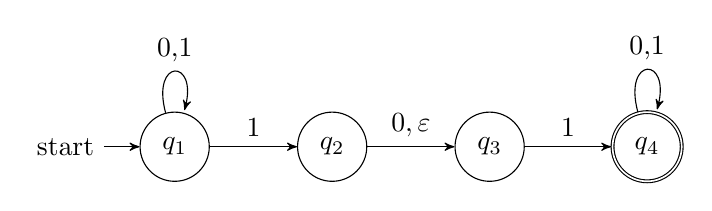
\begin{tikzpicture}
    \node[state, initial] (q1) {$q_1$};
    \node[state, right of=q1] (q2) {$q_2$};
    \node[state, right of=q2] (q3) {$q_3$};
    \node[state, accepting, right of=q3] (q4) {$q_4$};
    \draw (q1) edge[loop above] node{0,1} (q1)
          (q4) edge[loop above] node{0,1} (q4)
          (q1) edge[above] node{$1$} (q2)
          (q2) edge[above] node{$0,\varepsilon$} (q3)
          (q3) edge[above] node{$1$} (q4);
\end{tikzpicture}
\end{center}
\end{example}

The difference between a DFA and an NFA is immediately apparent. In the above example, there are multiple arrows from $q_1$ corresponding to input $1$ and no arrow from $q_2$ corresponding to $1$. We also see the addition of an $\varepsilon$ as input, which is not in the alphabet.
\vspace{3mm}
How does an NFA compute? At each point with multiple paths, the machine splits into multiple copies of itself, each one following one of the possibilites in parallel. Each copy of the machine then continues as before. If there are subsequent choices, it splits again. If the next input symbol does not appear on any of the arrows exiting the current state, that copy of the machine dies. Finally, if \textit{any} of these copies ends at an accept state, the NFA is said to accept the input string.

If a state with an $\varepsilon$ exiting arrow is encountered, the machine splits into multiple copies,each one following one of the arrows, \textit{without reading any input}.
\vspace{3mm}
Nondeterminism is a sort of parallel computing where many ``threads'' are running simultaneously. The NFA splitting corresponds to the process of ``forking'' into several children, each proceeding separately. If any of these processes accepts, the entire computation accepts.

We can also think of an NFA as a tree of possibilities where the tree splits at each point where the machine has more than one choice.
\vspace{3mm}

But why are NFA's important? As we shall see shortly, every NFA can be converted to an equivalent DFA, and constructing NFA's is sometimes easier than constructing DFA's. An NFA is usually much smaller than its DFA counterpart and its functioning may be easier to understand.

\begin{example}
Let $A$ be the language consisting of all strings over $\{0,1\}$ containing a $1$ in the third position from the end. The following NFA recognizes $A$.
\begin{center}
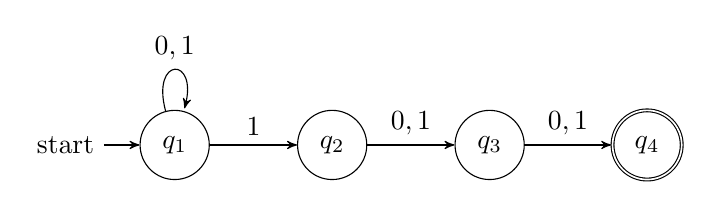
\begin{tikzpicture}
    \node[state, initial] (q1) {$q_1$};
    \node[state, right of=q1] (q2) {$q_2$};
    \node[state, right of=q2] (q3) {$q_3$};
    \node[state, accepting, right of=q3] (q4) {$q_4$};
    \draw (q1) edge[loop above] node{$0,1$} (q1)
          (q1) edge[above] node{$1$} (q2)
          (q2) edge[above] node{$0,1$} (q3)
          (q3) edge[above] node{$0,1$} (q4);
\end{tikzpicture}
\end{center}

The following DFA also recognizes $A$.
\begin{center}
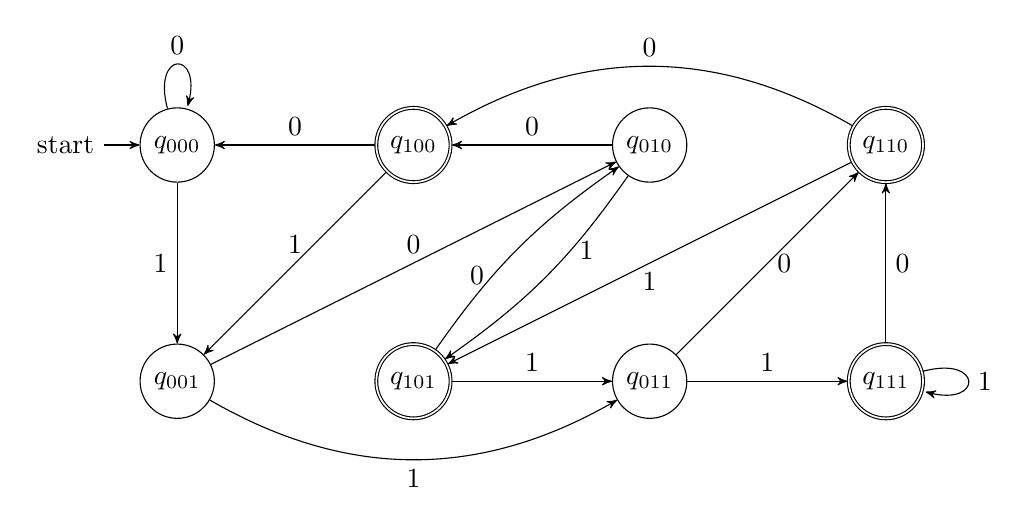
\begin{tikzpicture}[node distance=3cm]
    \node[state, initial] (q000) {$q_{000}$};
    \node[state, accepting, right of=q000] (q100) {$q_{100}$};
    \node[state, below of=q000] (q001) {$q_{001}$};
    \node[state, accepting, right of=q001] (q101) {$q_{101}$};
    \node[state, right of=q100] (q010) {$q_{010}$};
    \node[state, right of=q101] (q011) {$q_{011}$};
    \node[state, right of=q010, accepting] (q110) {$q_{110}$};
    \node[state, right of=q011, accepting] (q111) {$q_{111}$};
    \draw (q000) edge[loop above] node{0} (q000)
          (q111) edge[loop right] node{1} (q111)
          (q100) edge[above] node{0} (q000)
          (q000) edge[left] node{1} (q001)
          (q101) edge[above] node{1} (q011)
          (q011) edge[above] node{1} (q111)
          (q111) edge[right] node{0} (q110)
          (q010) edge[above] node{0} (q100)
          (q011) edge[right] node{0} (q110)
          (q101) edge[bend left=10, above, pos=0.25] node{0} (q010)
          (q010) edge[bend left=10, below, pos=0.25] node{1} (q101)
          (q001) edge[above] node{0} (q010)
          (q100) edge[above] node{1} (q001)
          (q110) edge[bend right, above] node{0} (q100)
          (q001) edge[bend right, below] node{1} (q011)
          (q110) edge[below] node{1} (q101);
\end{tikzpicture}
\end{center}
\end{example}

It is obvious that the DFA in the above example is far more complicated than the NFA.

Let us now formally define an NFA.
\begin{definition}
A nondeterministic finite automaton is a $5$-tuple $(Q,\Sigma,\delta,q_0,F)$, where
\begin{itemize}
    \item $Q$ is a finite set of states.
    \item $\Sigma$ is a finite alphabet.
    \item $\delta:Q\times\Sigma_\varepsilon\to\mathcal{P}(Q)$ is the transition function.
    \item $q_0\in Q$ is the start state, and
    \item $F\subseteq Q$ is the set of accept states.
\end{itemize}
\end{definition}

Here $\Sigma_\varepsilon$ is $\Sigma\cup\{\varepsilon\}$ and $\mathcal{P}(Q)$ is the power set of $Q$.
\vspace{3mm}
Let $w=y_1y_2\cdots y_m$ be a string over the alphabet $\Sigma$. We say that a nondeterministic finite automaton N \textit{accepts} $w$ if we can write $w$ as $w=y_1y_2\cdots y_m$ where each $y_i\in\Sigma_\varepsilon$ and a sequence of states $r=r_0,r_1,\ldots,r_m$ exists in $Q$ such that:
\begin{itemize}
    \item $r_0=q_0$,
    \item $r_{i+1}\in\delta(r_i, y_{i+1})$ for $i=0,1,\ldots,m-1$ and
    \item $r_m\in F$.
\end{itemize}

\begin{definition}
We say that two machines are \textit{equivalent} if they recognize the same language.
\end{definition}
\begin{theorem}
Every nondeterministic finite automaton has an equivalent deterministic finite automaton.
\end{theorem}

\begin{proof}
Let us first do this for the case where there are no $\varepsilon$ arrows. Then given an NFA $N=(Q,\Sigma,\delta,q_0,F)$ that recognizes language $A$, we can construct the DFA $M=(Q',\Sigma,\delta',q_0',F')$ such that
\begin{itemize}
    \item $Q'=\mathcal{P}(Q)$. $\mathcal{P}(Q)$ is the power set of $Q$.
    \item For any $R\in Q'$ and symbol $a$, $$\delta'(R,a)=\bigcup_{r\in R}\delta(r,a).$$
    \item $q_0'=\{q_0\}$.
    \item $F'=\{q\in Q\mid q\text{ contains at least one accept state}\}$.
\end{itemize}
Now we need to consider the $\varepsilon$ arrows as well. For any $R\in Q'$, define $$E(R)=\{q\mid q \text{ can be reached from $R$ by traveling along $0$ or more $\varepsilon$ arrows}\}.$$

We can then modify the transition function as follows:

$$\delta'(R,a)=\bigcup_{r\in R} E(\delta(r,a)).$$

We must also modify the start state to $q_0'=E(\{q_0\})$.

It is clear that this construction will work and recognize language $A$, as can easily be verified from the definition.
\end{proof}

Note that the size of the DFA created from the above construction equivalent to a given NFA has a number of nodes which is exponential in terms of the number of nodes of the NFA. It is thus clear why NFA's tend to be significantly more compact than their corresponding equivalent DFA's.

\begin{corollary}
A language is regular if and only if some nondeterministic finite automaton recognizes it.
\end{corollary}

Now that we have this much stronger corollary to determine if a language is regular, let us go back to continuing to prove that the class or regular languages is closed under the regular operations.

\begin{theorem}
The class of regular languages is closed under the union operation.
\end{theorem}
\begin{proof}
Let $N_1=(Q_1,\Sigma,\delta_1,q_1,F_1)$ recognize $A_1$ and $N_2=(Q_2,\Sigma,\delta_2,q_2,F_2)$ recognize $A_2$ for (regular) languages $A_1$ and $A_2$. (We assume that they have the same alphabet $\Sigma$. If they have different languages $\Sigma_1$ and $\Sigma_2$, set $\Sigma=\Sigma_1\cup\Sigma_2$).

Construct $N=(Q,\Sigma,\delta,q_0,F)$ to recognize $A_1\cup A_2$ as follows.
\begin{itemize}
    \item $Q=\{q_0\}\cup Q_1\cup Q_2$. (Assume without loss of generality that $Q_1$ and $Q_2$ are disjoint)
    \item The state $q_0$ is the start state of $N$. ($q_0$ is not in $Q_1$ or $Q_2$)
    \item $F=F_1\cup F_2$
    \item $\delta$ is defined as follows. For any $q\in Q$ and $a\in\Sigma_\varepsilon$,
    $$
    \delta(q,a)=
    \begin{cases}
    \delta_1(q,a) & q\in Q_1 \\
    \delta_2(q,a) & q\in Q_2 \\
    \{q_1,q_2\} & q=q_0\text{ and }a=\varepsilon \\
    \emptyset & q=q_0\text{ and }a\neq\varepsilon
    \end{cases}
    $$
\end{itemize}
Here we basically check separately whether a given string is accepted by $M_1$ or $M_2$, and accept if it is accepted by either.
\end{proof}

\begin{theorem}
The class of regular languages is closed under concatenation.
\end{theorem}
\begin{proof}
Let $N_1=(Q_1,\Sigma,\delta_1,q_1,F_1)$ recognize $A_1$ and $N_2=(Q_2,\Sigma,\delta_2,q_2,F_2)$ recognize $A_2$ for (regular) languages $A_1$ and $A_2$.

Construct $N=(Q,\Sigma,\delta,q_1,F_2)$ to recognize $A_1\circ A_2$.
\begin{itemize}
    \item $Q=Q_1\cup Q_2$.
    \item Define $\delta$ such that for any $q\in Q$ and $a\in\Sigma_\varepsilon$,
    $$
    \delta(q,a)=
    \begin{cases}
    \delta_1(q,a) & q\in Q_2\text{ and }q\not\in F_1 \\
    \delta_1(q,a) & q\in F_1\text{ and }a\neq\varepsilon \\
    \delta_1(q,a)\cup \{q_2\} & q\in F_1\text{ and }a=\varepsilon \\
    \delta_2(q,a) & q\in Q_2.
    \end{cases}
    $$
    We basically split if the part of the string read so far is accepted by $N_1$, check whether the remainder is accepted by $N_2$ and recurse.
\end{itemize}
\end{proof}

\begin{theorem}
The class of regular languages is closed under the star operation
\end{theorem}
\begin{proof}
Let $N_1=(Q_1,\Sigma,\delta_1,q_1,F_1)$ recognize $A$. Construct $N=(Q,\Sigma,\delta,q_0,F)$ as follows to recognize $A^*$.
\begin{itemize}
    \item $Q=\{q_0\}\cup Q_1$. ($q_0$ is not in $Q_1$)
    \item $F=\{q_0\}\cup F_1$. This is done so that $\varepsilon$ is in the resulting language.
    \item Define $\delta$ such that for any $q\in Q$ and any $a\in\Sigma_\varepsilon$,
    $$
    \delta(q,a)=
    \begin{cases}
    \delta_1(q,a) & q\in Q_1\text{ and }q\not\in F_1 \\
    \delta_1(q,a) & q\in F_1\text{ and }a\neq\varepsilon \\
    \delta_1(q,a)\cup\{q_1\} & q\in F_1\text{ and }a=\varepsilon \\
    \{q_1\} & q=q_0\text{ and }a=\varepsilon \\
    \emptyset & q=q_0\text{ and }a\neq\varepsilon
    \end{cases}
    $$
\end{itemize}

It can be checked that this machine recognizes $A^*$. The idea is similar to that in the concatenation proof, but we keep looping on the same machine.
\end{proof}

\begin{exercise}
Prove that the class of regular languages is closed under the intersection operation.
\end{exercise}
\clearpage

\subsection{Regular Expressions}
We use regular expressions to build up expressions describing languages, which are called regular expressions. An example is $(0\cup 1)\circ 0^*$. This language describes all strings that start with a $0$ or $1$ and are followed by $0$s. The concatenation symbol is usually omitted and understood implicitly, so the given expression can also be written as $(0\cup 1)0^*$.
\vspace{3mm}
Regular expressions have several obvious uses in computer science, like searching for strings in a text that satisfy certain properties for instance.

Like how in arithmetic, there is a precedence order in the operations wherein we give $\times$ and  higher precedence than $+$. Similarly, in regular expressions, the precedence order is star, then concatenation, and finally union. (unless parentheses are used to change the order)

\begin{definition}
We say that $R$ is a \textit{regular expression} if $R$ is
\begin{enumerate}
    \item $a$ for some $a$ in the alphabet $\Sigma$
    \item $\varepsilon$
    \item $\emptyset$
    \item $(R_1\cup R_2)$ for regular expressions $R_1$ and $R_2$
    \item $(R_1\circ R_2)$ for regular expressions $R_1$ and $R_2$
    \item $(R_1^*)$ for regular expression $R_1$.
\end{enumerate}
\end{definition}


\textit{Remark.} Do not confuse the regular expressions $\varepsilon$ and $\emptyset$. $\{\varepsilon\}$ is the language containing a single string, the empty string, whereas $\emptyset$ is the language containing no strings.
\vspace{3mm}
Given a regular expression $R$, we use $L(R)$ to denote the language of $R$.

For convenience, we use $R^+$ to denote $RR^*$, that is, the language has all strings that are $1$ or more concatenations of strings from $R$. So $R^+\cup\{\varepsilon\}=R^*$. We also let $R^k$ to denote the concatenation of $k$ $R$'s  with each other.

\begin{exercise}
Describe the languages corresponding to the following regular expressions.
\begin{enumerate}[(a)]
    \item $1^*\emptyset$
    \item $\emptyset^*$
    \item $(0\cup\varepsilon)(1\cup\varepsilon)$
    \item $(\Sigma\Sigma)^*$
    \item $(01^+)^*$
\end{enumerate}
\end{exercise}
\begin{solution}
~
\begin{enumerate}[(a)]
    \item $\emptyset$
    \item $\{\varepsilon\}$
    \item $\{\varepsilon,0,1,01\}$
    \item $\{w\mid w\text{ is a string of length }2\}$
    \item $\{w\mid \text{every $0$ in $w$ is followed by at least one $1$}\}$
\end{enumerate}
\end{solution}

\begin{exercise}
Prove the following identities for any regular language $R$.
\begin{enumerate}[(a)]
    \item $R\cup\emptyset=R$
    \item $R\circ\{\varepsilon\}=R$
\end{enumerate}
\end{exercise}

\vspace{3mm}

Regular expressions and finite automata are equivalent in their descriptive power, which may not be an immediately obvious fact. However any of them can be converted to the other.

\begin{lemma}
\label{regIfRegExp}
If a language is described by a regular expression, it is regular.
\end{lemma}
\begin{proof}
We shall prove each of the $5$ cases of the definition separately.
\begin{enumerate}
    \item $R=a$ for some $a$ in $\Sigma$. Then $L(R)=\{a\}$. The following NFA recognizes $L(R)$.
    \begin{center}
    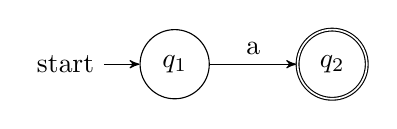
\begin{tikzpicture}
        \node[state, initial] (q1) {$q_1$};
        \node[state, accepting, right of=q1] (q2) {$q_2$};
        \draw (q1) edge[above] node{a} (q2);
    \end{tikzpicture}
    \end{center}
    
    \item $R=\varepsilon$. Then $L(R)=\{\varepsilon\}$. The following NFA recognizes $L(R)$.
    \begin{center}
    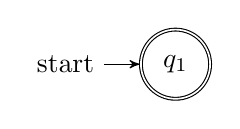
\begin{tikzpicture}
        \node[state, initial, accepting] (q1) {$q_1$};
    \end{tikzpicture}
    \end{center}
    
    \item $R=\emptyset$. Then $L(R)=\emptyset$. The following NFA recognizes $L(R)$.
    \begin{center}
    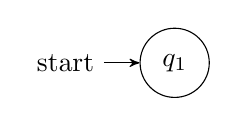
\begin{tikzpicture}
        \node[state, initial] (q1) {$q_1$};
    \end{tikzpicture}
    \end{center}
\end{enumerate}

For the remaining cases, that is, $R=R_1\cup R_2, R=R_1\circ R_2$ and $R=R_1^*$, we use the constructions given in the proofs that the regular languages are closed under each of the regular operations.
\end{proof}

We define a new type of automaton to help prove the next theorem, which states that if a language is regular, it can be described by a regular expression. We call this a generalized nondeterministic finite automaton (abbreviated as GNFA). The GNFA reads blocks of symbols from the input, not necessarily just one symbol at a time as in an ordinary NFA. The GNFA moves from one state to another by reading a block of symbols from the input, which may themselves constitute a string determined by the regular expression on that arrow.

For convenience, we also require that each GNFA always has a special form that meets the following criteria:
\begin{itemize}
    \item The start state has transition arrows going to every other state but no arrows coming in from any other state.
    \item There is only one accept state, and there are arrows coming in to the accept state from every other state but no arrows going out to any other state. Further, the accept state is not the same as the start state.
    \item Except for the start and accept states, there are arrows going from every state to every other state and also from each state to itself.
\end{itemize}

\label{regRegExpEquivSketch}
To prove the theorem, what we do is find a way to convert any DFA to a special GNFA (with $\geq 2$ states), and then repeatedly constructing an equivalent GNFA with $1$ less state by ``ripping'' out a state. When we get a GNFA with just 2 states, it just has a single arrow from the start state to the accept state, with label equal to the required regular expression.

\vspace{3mm}
Define $\mathcal{R}$ to be the set of all regular expressions over the alphabet $\Sigma$.

\begin{definition}
A \textit{generalized nondeterministic finite automaton} is a $5$-tuple $(Q,\Sigma,\delta,q_{\text{start}},q_{\text{accept}})$, where
\begin{itemize}
    \item $Q$ is the finite set of states,
    \item $\Sigma$ is the input alphabet,
    \item $\delta:(Q-\{q_{\text{accept}}\})\times(Q-\{q_{\text{start}}\})\to\mathcal{R}$ is the transition function,
    \item $q_{\text{start}}$ is the start state, and
    \item $q_{\text{accept}}$ is the accept state.
\end{itemize}
\end{definition}

A GNFA accepts a string $w$ in  $\Sigma^*$ if $w=w_1w_2\cdots w_k$, where each $w_i$ is in $\Sigma^*$  and a sequence of states $q_0,q_1,\ldots,q_k$ exist such that
\begin{itemize}
    \item $q_0=q_{\text{start}}$,
    \item $q_k=q_{\text{accept}}$, and
    \item for each $i$, we have $w_i\in L(R_i)$, where $R_i=\delta(q_{i-1},q_i)$. In other words, $R_i$ is the expression on the arrow from $q_{i-1}$ to $q_i$.
\end{itemize}

\begin{lemma}
\label{DFAtoSpGNFA}
Given any DFA, there exists an equivalent GNFA in the special form.
\end{lemma}
\begin{proof}
Consider a DFA $N=(Q,\Sigma,\delta,q_0,F)$, define a GNFA $N'=(Q',\Sigma,\delta',q_{\text{start}},q_{\text{accept}})$ as follows.
\begin{itemize}
    \item $Q'=Q\cup \{q_\text{start}, q_\text{accept}\}$, ($q_\text{start}$ and $q_\text{accept}$ are not in $Q$)
    \item $\delta'$ is defined as follows. For any $q_i,q_j\in Q'$,
    $$
    \delta'(q_i,q_j)=
    \begin{cases}
    \varepsilon & q_i=q_\text{start}\text{ and }q_j=q_0 \\
    \varepsilon & q_i\in F\text{ and } q_j=q_\text{accept} \\
    \{a: \delta(q_i,a)=q_j\} & \text{otherwise.}
    \end{cases}
    $$
\end{itemize}
    We simply add a new start state with an $\varepsilon$ arrow to the old start state, and a new accept state with $\varepsilon$ arrows from each of the old accept states. If any arrows have multiple labels, we replace these with a single arrow whose label is the union of the previous labels. We add arrows labelled $\emptyset$ between states that had no arrows between them.
    
    It can be checked that this is in fact a GNFA in special form.
\end{proof}

We shall now exactly describe the process that we use to obtain a regular expression from a given GNFA. Given a GNFA $G$, we define $\texttt{CONVERT}(G)$ by the following algorithm.

\begin{enumerate}
    \item Let $k$ be the number of states of $G$.
    
    \item If $k=2$, then $G$ must consist of a start state, an accept state, and exactly one arrow between them labelled with a regular expression $R$.
    
    Return $R.$
    
    \item If $k>2$, we select any state $q_{\text{rip}}\in Q$ different from $q_{\text{start}}$ and $q_{\text{accept}}$ and let $G'$ be the GNFA $(Q',\Sigma,\delta',q_{\text{start}},q_{\text{accept}})$ where
    $$Q'=Q-\{q_{\text{rip}}\},$$
    and for any $q_i\in Q'-\{q_{\text{accept}}\}$ and $q_j\in Q'-\{q_{\text{start}}\}$, let
    $$\delta'(q_i,q_j)=(R_1)(R_2)^*(R_3)\cup R_4$$
    for $R_1=\delta(q_i,q_\text{rip}), R_2=\delta(q_\text{rip}, q_\text{rip}), R_3=\delta(q_\text{rip},q_j)$ and $R_4=\delta(q_i,q_j)$.
    
    Return $\texttt{CONVERT}(G')$.  
\end{enumerate}

\begin{lemma}
\label{CONVERTeq}
For any GNFA $G$, $\texttt{CONVERT}(G)$ is equivalent to $G$.
\end{lemma}
\begin{proof}
We shall prove this by an induction on $k$, the number of states in $G$. Define $G'$ as in the above recursive algorithm.

\vspace{2mm}
\textit{Basis.} The basis case is $k=2$. In this case, $G$ only consists of a start state, an accept state, and a single arrow between them with the label describing all strings that $G$ recognizes. Thus the expression is equivalent to $G$.

\vspace{2mm}
\textit{Inductive step.} Assume it is true for $k-1$ states. Let $k>2$. We shall show that $G$, which has $k$ states, and $G'$, which has $k-1$ states, are equivalent, that is, they recognize the same language. Suppose that $G$ accepts a sequence $w$. Then in an accepting branch of the computation, $G$ enters a sequence of states $q_{\text{start}},q_1,q_2,\ldots,q_{\text{accept}}$.

If none of them is $q_{\text{rip}}$, $G'$ also clearly accepts $w$. If there are any runs of $q_{\text{rip}}$, then removing those runs also yields an accepting string. This is because for bracketing sequences $q_i,q_j$ around a run, the arrow between $q_i$ and $q_j$ has all strings from $q_i$ to $q_j$ through $q_\text{rip}$. So $G'$ accepts $w$.

On the other hand, if $G'$ accepts some sequence $w$, then the arrow from $q_i$ to $q_j$ in $G'$ describes the collection of strings taking $q_i$ to $q_j$ in $G$, either directly or through $q_\text{rip}$. Clearly, $G$ must also accept $w$. Thus $G$ and $G'$ are equivalent.

\vspace{2mm}
The induction hypothesis merely says that when the algorithm calls itself recursively on $G'$, the resulting regular expression is equivalent to $G'$ (because $G'$ has $k-1$ states). As $G$ is equivalent to $G'$, $G$ must also be equivalent to the resulting regular expression, namely $\texttt{CONVERT}(G)$.
\end{proof}
\vspace{1mm}
\begin{theorem}
\label{regIffRegExp}
A language is regular if and only if some regular expression describes it.
\end{theorem}
\begin{proof}
We have already proved one of the implications in \ref{regIfRegExp}.

To prove the other implication, we first use \ref{DFAtoSpGNFA} to create an equivalent GNFA given any DFA. We then use \ref{CONVERTeq} to obtain a regular expression that is equivalent to this GNFA, which is in turn equivalent to the initial DFA.

\vspace{2mm}
We thus have the two way implication.
\end{proof}

\vspace{1mm}
\begin{exercise}
Find the regular expression corresponding to the following NFA.
\begin{center}
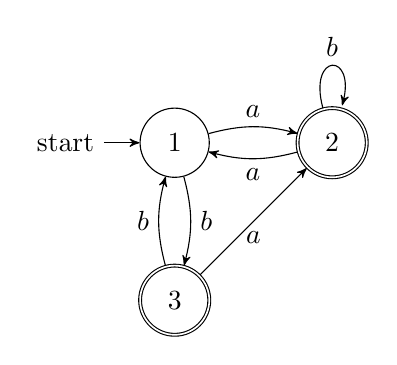
\begin{tikzpicture}
    \node[state, initial] (1) {$1$};
    \node[state, accepting, right of=1] (2) {$2$};
    \node[state, accepting, below of=1] (3) {$3$};
    \draw (1) edge[above, bend left=15] node{$a$} (2)
          (2) edge[below, bend left=15] node{$a$} (1)
          (2) edge[loop above] node{$b$} (2)
          (1) edge[right, bend left=15] node{$b$} (3)
          (3) edge[left, bend left=15] node{$b$} (1)
          (3) edge[below] node{$a$} (2);
\end{tikzpicture}
\end{center}
\end{exercise}
\begin{solution}
The resulting regular expression from the above DFA using the algorithm used in \ref{regIffRegExp} is
$$(a(aa\cup b)^*ab\cup b)((ba\cup a)(aa\cup b)^*ab\cup bb)^*((ba\cup a)(aa\cup b)^*\cup\varepsilon)\cup a(aa\cup b)^*$$
\end{solution}

\begin{exercise}
\label{stringreverse}
For any string $w=w_1w_2\cdots w_n$, the \textit{reverse} of $w$, written $w^\mathcal{R}$, is given by $w_n\cdots w_2w_1$. For any language $A$, denote $A^\mathcal{R}=\{w^\mathcal{R}\mid w\in A\}$. Show that if $A$ is regular, $A^\mathcal{R}$ is regular.
\end{exercise}
\clearpage

\subsection{Nonregular Languages}
As we have regular languages, the presence of \textit{nonregular} languages is also expected, that is, languages that cannot be recognized by any finite automaton. For instance, consider the language $B=\{0^n1^n\mid n\geq 0\}$. We wouldn't expect to have a finite automaton that recognizes this language as it appears we'd need to find a way to count the number of $0$s processed so far, and since this number is not bounded above and we only have a finite number of memory. Indeed, this language cannot be recognized by any finite automaton.

\vspace{2mm}
However, this immediately begs the question, what is a condition to determine whether a language is regular or nonregular? 

\begin{theorem}[The Pumping Lemma]
If $A$ is a regular language, then there is a number $p$, called the \textit{pumping length}, where if $s$ is any string in $A$ of length at least $p$, then $s$ can be divided into three pieces, $s=xyz$, satisfying the following conditions:
\begin{enumerate}
    \item For each $i\geq 0$, $xy^iz\in A$,
    \item $|y|>0$, and
    \item $|xy|\leq p$.
\end{enumerate}
\end{theorem}

The proof of this theorem essentially relies on the pigeonhole principle. If I set $p$ as the number of states, then I will have a segment in the middle which is just equal to a loop on some state. Since concatenating this segment with itself is still just a loop on that state, the theorem seems correct.

\begin{proof}
Let $M=(Q,\Sigma,\delta,q_0,F)$ be a DFA recognizing $A$. Let $p$ be the number of states of $M$.

Let $s=s_1s_2\cdots s_n$ be a string in $A$ of length $n\geq p$. Let $r_1,r_2,\ldots r_{n+1}$ be the corresponding states that $M$ goes through while processing $s$, so $r_{i+1}=\delta(r_i,s_i)$ for $i=1,2,\ldots,n$. As $M$ has $p$ states, we have that there is at least one repeated state in the first $p+1$ elements of the sequence (by the Pigeonhole principle). Let the indices of this repeated state be $l,j$, that is, $r_l=r_j$ where $l< j\leq p+1$. Set $x=s_1s_2\cdots s_{l-1}, y=s_ls_{l+1}\cdots s_{j-1}$ and $z=s_js_{j+1}\cdots s_n$. Now note that $x$ takes $M$ from $r_1$ to $r_l$, $y$ takes $M$ from $r_l$ to $r_l$, and $z$ takes $M$ from $r_l$ to $r_{n+1}$.

As $y$ takes $M$ from $r_l$ to $r_l$, $y^i$ for $i\geq 0$ will also take $M$ from $r_l$ to $r_l$ and $xy^iz$ will also be accepted by $M$. As $l\neq j$, $|y|>0$. And as $j\leq p+1, j-1\leq p$ and $|xy|\leq p$.
\end{proof}

\begin{exercise}
Prove that the language $B=\{0^n1^n\mid n\geq 0\}$ is nonregular.
\end{exercise}
\begin{solution}
If $B$ is a regular language, then consider $s=0^p1^p$, where $p$ is the pumping length. Let us take two cases. (Here $x,y,z$ represent the same $x,y,z$ as in the Pumping Lemma)
\begin{itemize}
    \item  $y$ is either only $0$s (or only $1$s). Then $xy^2z$ will have more $0$s ($1$s) than $1$s ($0$s) and so it is not in $B$.
    \item $y$ contains both $0$s and $1$s. Then $xy^2z$ can have the same number of $0$s and $1$s, but they will be out of order and hence it will not be a member of $B$.
\end{itemize}
We arrive at a contradiction and hence $B$ is not a regular language.
\end{solution}
\begin{exercise}
Prove that $B=\{w\mid w\text{ has an equal number of $0$s and $1$s}\}$ is a nonregular language.
\end{exercise}
\textit{Hint. }Show that $0^p1^p$ cannot be pumped.

\begin{exercise}
Prove the nonregularity of the following languages.
\begin{enumerate}[(a)]
    \item $D=\{ww\mid w\in\{0,1\}^*\}$.
    \item $E=\{1^{n^2}\mid n\geq 0\}$. This is a \textit{unary} nonregular language.
    \item $F=\{0^i1^j\mid i>j\}$.
\end{enumerate}
\end{exercise}

We shall now show another theorem that helps us determine when a language is regular.
\begin{definition}
Let $x$ and $y$ be strings and $L$ be any language. We say that $x$ and $y$ are \textit{distinguishable by $L$} if some string $z$ exists such that exactly one of the strings $xz$ and $yz$ is in $L$. Otherwise, if for every string $z$, $xz\in L$ if and only if $yz\in L$, we say that $x$ and $y$ are \textit{indistinguishable by $L$}.
\end{definition}

If $x$ and $y$ are indistinguishable by $L$, we write $x\equiv_Ly$.
\begin{lemma}
Given a language $L$, $\equiv_L$ is an equivalence relation.
\end{lemma}
\begin{proof}
This proof is trivial and is left as an exercise to the reader.
\end{proof}

\begin{definition}
Let $L$ be a language and $X$ be a set of strings. We say that $X$ is \textit{pairwise distinguishable} by $L$ if every two distinct strings in $X$ are distinguishable by $L$. 
\end{definition}
\begin{definition}
Let $L$ be a language. The \textit{index} of $L$ is defined as the maximum number of elements in any set that is pairwise distinguishable by $L$. The index of a language may be finite or infinite.
\end{definition}
\begin{theorem}[Myhill-Nerode Theorem]
A language $L$ is regular if and only if it has finite index. Moreover, its index is the size of the smallest DFA recognizing it.
\end{theorem}
\begin{proof}
We shall first show that if a language $L$ is recognized by a DFA with $k$ states, it has index at most $k$.

If there exists a set with $> k$ elements that is pairwise distinguishable, then by the Pigeonhole principle, we get that there exist two strings $x$ and $y$ in the set such that the state the DFA is in after processing these strings is the same. However, if this is the case, then for any string $z$, the DFA will accept $xz$ if and only if it accepts $yz$. Thus, the index is at most $k$.

\vspace{2mm}
We shall now show the other direction, that is, if the index of $L$ is a finite number $k$, it is recognized by a DFA with $k$ states.

Let $X=\{x_1,x_2,\ldots,x_k\}$ be pairwise distinguishable by $L$. Construct a DFA $N=\{Q,\Sigma,\delta,x_0,F\}$ as follows. $Q=X$. $\delta(x_i,a)=x_j$ if $x_ia\equiv_Lx_j$. Note that this $x_j$ is unique as $X$ is pairwise distinguishable and such an $x_j$ exists as $X$ has the \textit{maximum} number of elements. $x_0$ is the unique $x_i$ such that $x_i\equiv_L\varepsilon$. $F=X\cap L$. If a string $s\equiv_Lx_j$ for some $j$, then the state of $N$ after reading $s$ will be $x_j$ (Why?). Thus the language recognized by $N$ is just $L$ itself (from the definition of $F$).

\vspace{2mm}
Combining the above two, we get that a language is regular if and only if it has finite index. To prove the second part of the theorem, suppose that there is a DFA that recognizes the language with size less than the index. Then using the first part of the proof gives a contradiction. There clearly exists a DFA recognizing the language of size equal to the index from the second part of the theorem. This completes our proof.
\end{proof}
\clearpage

\subsection*{Problems}

\begin{exercise}
Let
$$\Sigma_3=\left\{\begin{bmatrix}0\\0\\0\end{bmatrix}, \begin{bmatrix}0\\0\\1\end{bmatrix}, \begin{bmatrix}0\\1\\0\end{bmatrix},\cdots,\begin{bmatrix}1\\1\\1\end{bmatrix}\right\}.$$
A string in $\Sigma_3$ gives $3$ rows. Consider each row to be a binary number and let
$$B=\{w\in\Sigma_3^*\mid \text{the bottom row of $w$ is the sum of the top two rows}\}$$
Show that $B$ is regular.
\end{exercise}

\begin{exercise}
\label{LwwR}
Consider the language
$$L=\{ww^\mathcal{R}\mid w\in (0\cup 1)^*\}$$
Show that $L$ is nonregular. (The meaning of $w^\mathcal{R}$ is described in \ref{stringreverse}.)
\end{exercise}

\begin{exercise}
Say that string $x$ is a \textit{prefix} of string $y$ if a string $z$ exists such that $xz=y$ and that $x$ is a \textit{proper prefix} of $y$ if in addition, $x\neq y$. Let $A$ be any language. Show that the class of regular languages is closed under the following two operations.
\begin{enumerate}[(a)]
    \item $\texttt{NOPREFIX}(A)=\{w\in A\mid \text{no proper prefix of $w$ is in $A$}\}$
    \item $\texttt{NOEXTEND}(A)=\{w\in A\mid w\text{ is not the proper prefix of any string in $A$}\}$
\end{enumerate}
\end{exercise}

\begin{exercise}
Let $A$ be any language. Show that the class of regular languages is closed under the $\texttt{DROPOUT}$ operation defined as follows.
$$\texttt{DROPOUT}(A)=\{xz\mid xyz\in A\text{ where }x,z\in\Sigma^*,y\in\Sigma\}.$$
\end{exercise}

\begin{exercise}
For languages $A$ and $B$, let the shuffle of $A$ and $B$ be the language
$$\{w\mid w=a_1b_1\cdots a_kb_k,\text{ where $a_1\cdots a_k\in A$ and $b_1\cdots b_k\in B$, each $a_i,b_i\in\Sigma^*$}\}.$$
Show that the classes of regular languages is closed under the shuffle operation.
\end{exercise}

\begin{exercise}
If $A$ is any language, let $A_{\frac 12-}$ be the set of all first halves of strings in $A$ defined as follows.
$$A_{\frac 12-}=\{x\mid \text{for some }y, |x|=|y|\text{ and }xy\in A\}$$
Show that if $A$ is regular, so is $A_{\frac 12-}$.
\end{exercise}

\begin{exercise}
Let $B$ and $D$ be two languages. Write $B\Subset D$ if $B\subseteq D$ and $D$ contains infinitely many strings that are not in $B$. Show that, if $B$ and $D$ are two regular languages where $B\Subset D$, then we can find a regular language $C$ where $B\Subset C\Subset D$.
\end{exercise}

\begin{exercise}
Let $M=\{Q,\Sigma,\delta,q_0,F\}$ be a DFA and $h\in Q$ be called its ``home''. A \textit{synchronizing sequence} for $M$ and $h$ is a string $s\in\Sigma^*$ where $\hat\delta(q,s)=h$ for all $q\in Q$ (Here $\hat\delta(q,s)$ is the state $M$ ends up at when it starts at $q$ and processes $s$). Say that $M$ is \textit{synchronizable} if it has a synchronizing sequence for some state $h$. Prove that if $M$ is a $k$-state synchronizable DFA, it has a synchronizing sequence of length at most $k^3$.

This has in fact been improved by Kohavi (?, check again) to show that the length of the synchronizing sequence lies between $\frac{k^3-k}{6}$ and $\frac{k^2+k-4}{2}$. \u{C}ern\'{y} conjectured in 1964 that this bound can be improved to $(k-1)^2$, a very tight bound, which remains one of the largest unsolved problems in Automata Theory at the time of writing this.
\end{exercise}
\clearpage

\section{Context-Free Languages}
In this chapter, we shall present context-free grammars, that can describe certain features that have a recursive structure. They naturally arise from trying to understand the relationship of terms like nouns, verbs and prepositions in ordinary grammar, and their respective phrases which lead to a natural recursion.

An important application of this is in most compilers and interpreters, which contain a parser that extracts the meaning of a program prior to compilation. A number of methods help construct this parser once a context-free language is available. Some even automatically generate the parser.

The collection of associated languages are \textit{context-free languages}.

\subsection{Context-Free Grammars}

\begin{example}
The following is a context-free grammar. Call it $G_1$.
\begin{align*}
    A &\to 0A1 \\
    A &\to B \\
    B &\to \#
\end{align*}
The grammar consists of \textit{substitution rules} or \textit{productions}. Each rule has a symbol, called a \textit{variable}, and a string separated by an arrow. The string contains variables and other symbols called \textit{terminals}. One variable is designated as the start variable, and usually occurs on the left-hand side of the top-most rule. Using a grammar, we describe a language, called a context-free language, by generating each string of that language as follows.
\begin{enumerate}
    \item Write down the start variable.
    \item Find a variable that is written down and a rule that starts with that variable. Replace that variable with the right hand side of that rule.
    \item Repeat step $2$ until no more variables remain.
\end{enumerate}
For example, $G_1$ generates $00\# 11$ as follows.
$$A\implies 0A1\implies 00A11\implies 00B11\implies 00\# 11$$
\end{example}

\bigskip
The above information may also be represented pictorially by a \textit{parse tree}.

\vspace{3mm}
In the above example, the two rules with $A$ on the left-hand side can be merged into a single rule as  $A\to 0A1\mid B$, using the symbol ``$|$" as an ``or". To understand the link with the English language, we give a more illustrative example below.
\begin{example}
\begin{align*}
    \langle\texttt{SENTENCE}\rangle &\to \langle\texttt{NOUN-PHRASE}\rangle\langle\texttt{VERB-PHRASE}\rangle \\
    \langle\texttt{NOUN-PHRASE}\rangle &\to \langle\texttt{CMPLX-NOUN}\rangle\mid\langle\texttt{CMPLX-NOUN}\rangle\langle\texttt{PREP-PHRASE}\rangle \\
    \langle\texttt{VERB-PHRASE}\rangle&\to\langle\texttt{CMPLX-VERB}\rangle\mid\langle\texttt{CMPLX-VERB}\rangle\langle\texttt{PREP-PHRASE}\rangle \\
    \langle\texttt{PREP-PHRASE}\rangle&\to\langle\texttt{PREP}\rangle\langle\texttt{CMPLX-NOUN}\rangle \\
    \langle\texttt{CMPLX-NOUN}\rangle&\to\langle\texttt{ARTICLE}\rangle\langle\texttt{NOUN}\rangle \\
    \langle\texttt{CMPLX-VERB}\rangle&\to\langle\texttt{VERB}\rangle\mid\langle\texttt{VERB}\rangle\langle\texttt{NOUN-PHRASE}\rangle \\
    \langle\texttt{ARTICLE}\rangle&\to\texttt{a}\mid\texttt{the} \\
    \langle\texttt{NOUN}\rangle&\to\texttt{boy}\mid\texttt{girl}\mid\texttt{flower} \\
    \langle\texttt{VERB}\rangle&\to\texttt{touches}\mid\texttt{sees}\\
    \langle\texttt{PREP}\rangle&\to\texttt{with}
\end{align*}

Strings in this grammar include\\
\quad \texttt{a boy sees} \\    
\quad \texttt{the boy touches a flower} \\
\quad \texttt{the girl touches the boy with the flower}
\end{example}

\begin{exercise}
Show two different ways in which the third string in the above grammar can be generated. Here, ``two different ways" means two different parse trees, not two different derivations. (Why aren't these two the same?) Note the correspondence between these two ways and the two ways the string can be read.
\end{exercise}

\vspace{3mm}
Let us formalize our definition of a context-free grammar.
\begin{definition}
A \textit{context-free grammar} is a $4$-tuple $(V,\Sigma,R,S)$, where
\begin{enumerate}
    \item $V$ is a finite set called the \textit{variables}.
    \item $\Sigma$ is a finite set, disjoint from $V$, called the \textit{terminals}.
    \item $R$ is a finite set of \textit{rules}, with each rule being a variable and a string of variables and terminals. More precisely, $R$ is a finite subset of $V\times (V\cup\Sigma)^*$, called the \textit{set of rules}.
    \item $S\in V$ is the \textit{start variable}.
\end{enumerate}
\end{definition}

We shall abbreviate ``context-free grammar" as CFG and ``context-free language" as CFL.

If $u,v$ and $w$ are strings of variables and terminals, and $A\to w$ is a rule of the grammar, we say that $uAv$ \textit{yields} $uwv$, written as $uAv\yields uwv$.

We say that $u$ \textit{derives} $v$, written $u\derives v$, if $u=v$ or there exists a sequence $u_1,u_2,\ldots,u_k$ of strings of terminals and variables some for $k\geq 0$ such that $$u\yields u_1\yields u_2 \yields\cdots\yields u_k\yields v$$

The \textit{language} of the grammar is $\{w\in\Sigma^*\mid S\derives w\}$.

\begin{exercise}
Put the two examples given above in the form given in the definition of a CFG.
\end{exercise}

Many CFLs are the union of simpler CFLs. These can then easily be combined to form a corresponding CFG by combining their rules and then adding a new rule $S\to S_1\mid S_2\mid\cdots\mid S_k$, where the $S_i$s are the start variables of each of the CFGs.

\begin{exercise}
Construct a CFG which has corresponding language $\{0^n1^n\mid n\geq 0\}\cup\{1^n0^n\mid n\geq 0\}$
\end{exercise}
\begin{solution}
We can combine the two following CFGs:
$$S_1\to 0S_11\mid\varepsilon \text{ and } S_2\to 1S_20\mid\varepsilon$$
to get a grammar that generates the given language as follows.
\begin{align*}
    S&\to S_1\mid S_2 \\
    S_1&\to 0S_11\mid\varepsilon \\
    S_2&\to 1S_20\mid\varepsilon
\end{align*}
\end{solution}

\begin{lemma}
Any regular language is a context-free language.
\end{lemma}
\begin{proof}
Let $N(Q,\Sigma,\delta,q_0,F)$ be a DFA that recognizes the given regular language. We convert $N$ to a CFG $G(V,\Sigma,R,S)$ as follows.
\begin{itemize}
    \item $V=Q$
    \item $R=\{q_i\to aq_j\mid q_i,q_j\in V \text{ and } \delta(q_i,a)=q_j\} \cup\{q_i\to\varepsilon\mid q_i\in F\}$
    \item $S=q_0$
\end{itemize}
We leave it to the reader to verify that this grammar generates the language of the DFA.
\end{proof}

If a grammar generates a string in multiple ways, we say that the string is generated ambiguously from the grammar.
\begin{definition}
A derivation of a string in a grammar $G$ is a \textit{leftmost derivation} if at every step the leftmost remaining variable is replaced.
\end{definition}

Rightmost derivations are defined similarly.

\begin{definition}
Let $(V,\Sigma,R,S)$ be a context-free grammar. Any string in $(V\cup\Sigma)^*$ that can be derived from the start symbol $S$ is called a \textit{sentential form}.
\end{definition}

In the above definition, if there exists a leftmost derivation from $S$ to the sentential form, it is called a \textit{left-sentential form}. Right-sentential forms are defined similarly.

\begin{definition}
A string $w$ is derived \textit{ambiguously} in a context-free grammar $G$ if it has two or more different left-most derivations. Grammar $G$ is \textit{ambiguous} if it generates some string ambiguously.
\end{definition}

Sometimes when we have an ambiguous grammar, we can find an unambiguous grammar that generates the same language. Some languages, however, can only be generated by ambiguous grammars. Such languages are called \textit{inherently ambiguous}.

\vspace{3mm}
It is often very useful to represent context-free grammars in a simplified form.

\begin{definition}
A context-free grammar is in \textit{Chomsky normal form} if every rule is of the form
\begin{align*}
    A&\to BC \\
    A&\to a
\end{align*}
where $a$ is any terminal, $A$ is any variable and $B,C$ are any variable other than the start variable. In addition, we permit the rule $S\to\varepsilon$, where $S$ is the start variable.
\end{definition}

\begin{theorem}
Any context-free language can be generated by a context-free grammar in Chomsky normal form.
\end{theorem}
\begin{proof}
We can convert any CFG $G$ into Chomsky normal form as follows.

\begin{enumerate}
    \item Add a new variable $S_0$ and the rule $S_0\to S$, where $S$ was the original start variable. This is done to ensure that the start variable is not on the right side of any rule.
    \item Next, we take care of all $\varepsilon$-rules, that is, rules with $\varepsilon$ on the right side. We remove any $\varepsilon$-rule $A\to\varepsilon$, where $A\neq S$. Then for each occurrence of $A$ on the right side of a rule, we add a new rule with that occurrence deleted. We repeat this until there are no $\varepsilon$ rules not involving $S$.
    \item We then handle all unit rules. We remove a unit rule $A\to B$. Then wherever a rule $B\to u$ appears, we add the rule $A\to u$ unless this was a unit rule previously removed. Here, $u$ is a string of variables and terminals. We repeat this until there are no unit rules.
    \item Given any rule $A\to u_1u_2\cdots u_k$, where $k>2$ and each $u_i$ is a variable or terminal symbol, with the rules $A\to u_1A_1, A_1\to u_2A_2, \ldots,$ and $A_{k-2}\to u_{k-1}u_k$ (The $A_i$s  are new variables).
    \item Finally, if we have any rule $A\to u_1u_2$, we replace any terminal $u_i$ with the new variable $U_i$ and add the rule $U_i\to u_i$.
\end{enumerate}

It can be checked that the language of this grammar is the same as that of the original grammar.
\end{proof}

\begin{exercise}
Convert to the following CFG to Chomsky normal form.
\begin{align*}
    S&\to ASA\mid aB \\
    A&\to B\mid S \\
    B&\to b\mid\varepsilon
\end{align*}
\end{exercise}
\begin{solution}
Performing the algorithm given in the above proof yields the following CFG.
\begin{align*}
    S_0&\to AA_1\mid UB\mid a\mid SA\mid AS \\
    S&\to AA_1\mid UB\mid a\mid SA\mid AS \\
    A&\to b\mid AA_1\mid UB\mid a\mid SA\mid AS \\
    A_1&\to SA \\
    U&\to a \\
    B&\to b \\
\end{align*}
\end{solution}
\clearpage

\subsection{Pushdown Automata}
We shall now introduce another computational model called a \textit{pushdown automaton}. These automata are like DFAs, but they have an extra component called a \textit{stack}, which provides additional memory beyond that of just the DFA. This allows the automaton to recognize certain non-regular languages. Pushdown automata are equivalent in power to context-free grammars. 

The schematic of a finite automaton can be understood as follows:
\begin{center}
\begin{tikzpicture}[block_center/.style ={rectangle, draw=black, fill=white, text width=7em, text centered, minimum height=4em}, cell/.style={rectangle,draw=black},
space/.style={minimum height=1.5em,matrix of nodes,row sep=-\pgflinewidth,column sep=-\pgflinewidth,column 1/.style={font=\ttfamily}},text depth=0.5ex,text height=2ex,nodes in empty cells]
    \node[block_center] (control) {state control};
    
    \matrix (input) [space, below right=0.2cm and 3cm of control, column 1/.style={nodes={cell,minimum width=2em}},column 2/.style={nodes={cell,minimum width=2em}},column 3/.style={nodes={cell,minimum width=2em}},column 4/.style={nodes={cell,minimum width=2em}}]
    {
    a & b & b & a \\};
    
    \node[below=0.1cm of input] {input};
    \draw (control) -| (input-1-1);
    \end{tikzpicture}
\end{center}

The ``state control" represents the states and the transition function, and the tape contains the input string, which is read character by character. The arrow points at the next character to be read.

\vspace{3mm}
Similarly, a pushdown automaton can be understood as follows.

\begin{center}
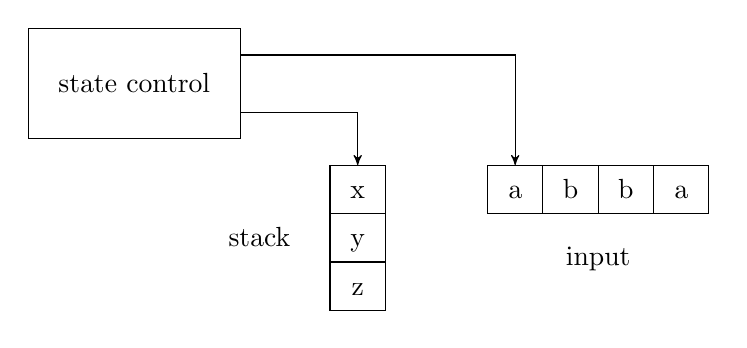
\begin{tikzpicture}[block_center/.style ={rectangle, draw=black, fill=white, text width=7em, text centered, minimum height=4em}, cell/.style={rectangle,draw=black},
space/.style={minimum height=1.5em,matrix of nodes,row sep=-\pgflinewidth,column sep=-\pgflinewidth,column 1/.style={font=\ttfamily}},text depth=0.5ex,text height=2ex,nodes in empty cells]
    \node[block_center] (control) {state control};
    
    \matrix (input) [space, below right=0.2cm and 3cm of control, column 1/.style={nodes={cell,minimum width=2em}},column 2/.style={nodes={cell,minimum width=2em}},column 3/.style={nodes={cell,minimum width=2em}},column 4/.style={nodes={cell,minimum width=2em}}]
    {
    a & b & b & a \\};
    
    \matrix (stack) [space, below right=0.2cm and 1cm of control, column 1/.style={nodes={cell,minimum width=2em}}]
    {
    x \\ y \\ z \\};

    \node[left=0.25cm of stack] {stack};
    \node[below=0.1cm of input] {input};
    \draw (control.15) -| (input-1-1);
    \draw (control.-15) -| (stack-1-1);
\end{tikzpicture}
\end{center}

In addition to the finite automaton-like structure it has, it also has a stack on which which symbols can be written down and read back later (The concept of a stack is hopefully familiar to the reader). This stack, which has infinite memory, is what enables the pushdown automaton to recognize languages such as $\{0^n1^n\mid n\geq 0\}$ because it can store the number of $0$s it has seen on the stack. The ``pushdown" in pushdown automaton corresponds to the stack structure.

\vspace{3mm}
Unlike DFAs and NFAs, deterministic pushdown automata and nondeterministic pushdown automata are \textit{not} equivalent. However, as nondeterministic pushdown automata are equivalent to context-free grammars, we shall focus on them for the remainder of this subsection.

\begin{example}
Let us attempt to construct the pushdown automaton corresponding to the language $L$ described in \ref{LwwR}. We do so as follows.
\begin{itemize}
    \item Start in a state $q_0$ that represents a guess that we have not yet seen the end of the $w$ in the definition of $L$. While in state $q_0$, we read symbols and push them onto the stack.
    \item At any time, we may guess that we have reached the end of $w$. Since the automaton is nondeterministic, we guess that we have reached the end of $w$ by going to state $q_1$, and also stay in $q_0$ and continue to read inputs.
    \item Once in state $q_1$, we look at the input symbol and compare it to the topmost symbol on the stack. If they are the same, we pop it. Otherwise, the branch dies.
    \item If we empty the stack, then we have seen something of the form $ww^\mathcal{R}$, so we accept.
\end{itemize}
\end{example}

\vspace{3mm}
We shall now formally define a nondeterministic pushdown automaton.
\begin{definition}
A \textit{nondeterministic pushdown automaton} is a $7$-tuple $(Q,\Sigma,\Gamma,\delta,q_0,Z_0,F)$ where $Q,\Sigma, \Gamma, F$ are all finite sets, and
\begin{enumerate}
    \item $Q$ is the (finite) \textit{set of states},
    \item $\Sigma$ is the (finite) \textit{input alphabet},
    \item $\Gamma$ is the (finite) \textit{stack alphabet} (this is the set of elements we can push onto the stack),
    \item $\delta:Q\times\Sigma_\varepsilon\times\Gamma\to\mathcal{P}(Q\times\Gamma^*)$ is the \textit{transition function},
    \item $q_0\in Q$ is the \textit{start state},
    \item $Z_0\in\Gamma$ is a particular symbol called the \textit{start symbol}, which initially appears on the stack, and
    \item $F\subseteq Q$ is the \textit{set of accept states}.
\end{enumerate}
\end{definition}

\vspace{2mm}
We shall abbreviate ``Nondeterministic Pushdown Automaton" as NPDA.

In the above definition, the transition function is the main thing that is different from our usual definition of an NFA. In one transition, it:
\begin{enumerate}
    \item consumes from input the symbol used in the transition (if the symbol is $\varepsilon$, then no input is consumed),
    \item goes to a new state, and
    \item replaces the symbol at the top of the stack with a string. Note that the string could also be $\varepsilon$, which means that we pop the stack.
\end{enumerate}
Given this, the correspondence to the above definition is clear.

We require $Z_0$ in the above definition of a stack so that we can know when the stack is empty. Note that it is equivalent to use a specific symbol that we push in the beginning to signify the bottom of the stack. Some books use this definition of the NPDA instead. Next, we shall define what it means for an NPDA to recognize a string.

\begin{definition}
An NPDA $M=\writeNPDA$ is said to \textit{accept} a string $w$ if $w$ can be written as $w=w_1w_2\cdots w_m$, where each $w_i\in\Sigma_\varepsilon$ and sequence of states $r_0,r_1,\ldots,r_m\in Q$ and strings $s_0,s_1,\ldots,s_m\in\Gamma^*$ exist that satisfy the following three conditions.
\begin{enumerate}
    \item $r_0=q_0$ and $s_0=Z_0$.
    \item For $i=0,1,\ldots,m-1$, we have $(r_{i+1},b)\in\delta(r_i,w_{i+1},a)$, where $s_i=at$ and $s_{i+1}=bt$ for some $a\in\Gamma$ and $b,t\in\Gamma^*$.
    \item $r_m\in F$.
\end{enumerate}
\end{definition}

\begin{exercise}
\label{LwwRexercise}
Express the example we described before defining an NPDA in the form given in the definition of an NPDA.
\end{exercise}
\begin{solution}
The PDA can be expressed as $P=(\{q_0,q_1,q_2\}, \{0,1\}, \{0,1,Z_0\}, \delta, q_0,Z_0, \{q_2\})$, where
\begin{align*}
    \delta(q_0,a,Z_0) &= \{(q_0,aZ_0)\}\quad\text{for all $a\in\{0,1\}$} \\
    \delta(q_0,a,b) &= \{(q_0,ab)\}\quad\text{for all $a,b\in\{0,1\}$} \\
    \delta(q_0,\varepsilon,a) &= \{(q_1,a)\}\quad\text{for all $a\in\{0,1,Z_0\}$} \\
    \delta(q_1,a,a) &= \{(q_1,\varepsilon)\}\quad\text{for all $a\in\{0,1\}$} \\
    \delta(q_1,\varepsilon,Z_0) &= \{(q_2,Z_0)\}
\end{align*}
\end{solution}
    
\vspace{3mm}
Similar to how we express NFAs and DFAs as graphs, NPDAs can also be expressed as graphs, where in addition to the way we draw the NFA structure, we also write what happens to the stack as follows. An arc labelled $a,X/\alpha$ from state $q$ to $p$ means that $(p,\alpha)\in\delta(q,a,X)$. That is, it tells what input is used ($a$), and the old and new tops of the stack ($X$ and $\alpha$ respectively).

\vspace{3mm}
So for instance, the PDA described in \ref{LwwRexercise} is depicted by the following diagram.

\begin{center}
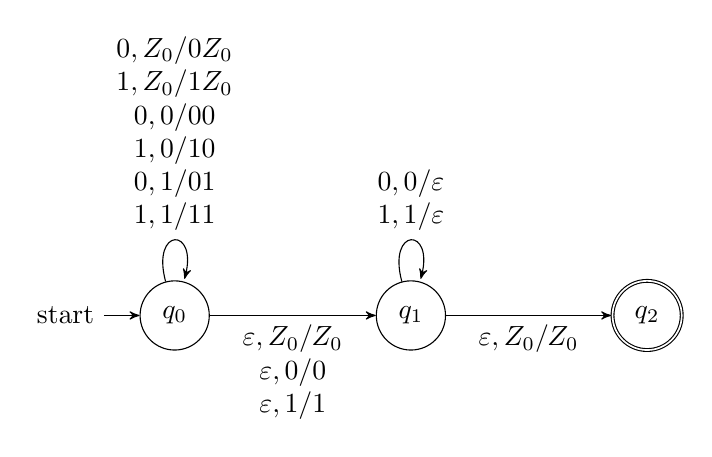
\begin{tikzpicture}[node distance=3cm]
    \node[state,initial] (q0) {$q_0$};
    \node[state,right of=q0] (q1) {$q_1$};
    \node[state,accepting,right of=q1] (q2) {$q_2$};
    \draw (q0) edge[loop above] node[align=center] {$0,Z_0/0Z_0$ \\ $1,Z_0/1Z_0$        \\ $0, 0/00$ \\ $1, 0/10$ \\ $0, 1/01$ \\ $1, 1/11$} (q0)
          (q1) edge[loop above] node[align=center]{$0, 0/\varepsilon$ \\ $1, 1/\varepsilon$} (q1)
          (q0) edge[below] node[align=center] {$\varepsilon, Z_0/Z_0$ \\ $\varepsilon, 0/0$ \\ $\varepsilon, 1/1$} (q1)
          (q1) edge[below] node[align=center] {$\varepsilon, Z_0/Z_0$} (q2);
\end{tikzpicture}
\end{center}

\begin{exercise}
Construct the NPDA that recognizes the language $L=\{a^ib^jc^k\mid i=j\text{ or }j=k\}$
\end{exercise}

It is also useful to represent a PDA at some point of time by a triple $(q,w,\gamma)$, where $q$ is the state, $w$ is the remaining input, and $\gamma$ is the stack contents. We conventionally show the top of the stack at the left end of $\gamma$. Such a triple is called an \textit{instantaneous description}, or ID of the automaton.

\vspace{3mm}
Let $V=\writeNPDA$ be an NPDA. Define $\vdash_P$, or just $\vdash$ when $P$ is understood, as follows. Suppose $(p,\alpha)\in\delta(q,a,X)$. Then for all strings $w\in\Sigma^*,\beta\in\Gamma^*$, we write
$$(q,aw,X\beta)\vdash(p,w,\alpha\beta)$$
This notation, called the \textit{``turnstile"} notation, represents the transition between different IDs of the NPDA. Note that $w$ and $\beta$ do not influence the transition, they are merely carried along.

We also use $\vdash^*_P$ or $\vdash^*$ to represent $0$ or more moves of the NPDA. That is, $I\vdash^* I$ for any ID $I$ and $I\vdash J$ if there exists a state $K$ such that $I\vdash K$ and $K\vdash^* J$.

\vspace{3mm}
We shall call a sequence of IDs a \textit{computation}. We have the following.
\begin{itemize}
    \item If a computation is legal, then the computation formed by adding the same additional input string to the end of the input in each ID is also legal.
    \item If a computation is legal, then the computation formed by adding the same additional string below the stack of each ID is also legal.
    \item If a computation is legal, and some tail of the input is not consumed, we can remove this tail from each ID and the resulting computation will still be legal.
\end{itemize}

These three points just say that information that the NPDA does not look at does not affect its computation.

\begin{theorem}
\label{dontreaddontcare}
If $P=\writeNPDA$ is an NPDA and $(q,x,\alpha)\vdash^*_P(p,y,\beta)$, then for any strings $w\in\Sigma^*, \gamma\in\Gamma^*$, $$(q,xw,\alpha\gamma)\vdash^*_P(p,yw,\beta\gamma).$$
\end{theorem}
\begin{proof}
This proof is trivial and is left as an exercise to the reader. (Perform an induction on the number of steps in the sequence of IDs)
\end{proof}

Using this notation, we can alternatively formulate the definition of the language recognized by a language as follows.
Let $P=\writeNPDA$ be an NPDA. Then
$$L(P)=\{(q_0,w,Z_0)\vdash^*_P(q,\varepsilon,\alpha)\mid q\in F\text{ and }\alpha\in\Gamma^*\}$$
The above condition is called \textit{acceptance by final state}, which is exactly what it is.
\begin{definition}
Let $P=\writeNPDA$ be an NPDA. We define
$$N(P)=\{w\mid (q_0,w,Z_0)\vdash^*(q,\varepsilon,\varepsilon)\}$$
\end{definition}


The above set represents the set of input strings that when consumed, empty the stack as well. This is called \textit{acceptance by empty stack}.

The following two theorems shows how the above two acceptances are intimately related.

\begin{lemma}
\label{finalifemptystk}
If $L=N(P_N)$ for some NPDA $P_N=(Q,\Sigma,\Gamma,\delta_N,q_0,Z_0)$, then there is an NPDA $P_F$ such that $L(P_F)=L$.
\end{lemma}
\begin{proof}
We first set the start symbol of $P_F$ as some $X_0\not\in\Gamma$. If we see $X_0$ on the stack for some input, then it means that $P_N$ would empty the stack for that same input. We also set the start state of $P_F$ as some $p_0\not\in Q$, whose sole purpose is to push $Z_0$ onto the stack and send it to $q_0$. Then, $P_F$ simulates $P_N$, until the stack of $P_N$ is empty. We also create another state $p_f\not\in Q$, which is the (unique) accepting state of $P_F$. $P_F$ goes to $p_f$ if $P_N$ would have emptied the stack for that input (that is, it has $X_0$ on the top of the stack).

%ADD DIAGRAM!
That is, $$P_F=(Q\cup\{p_0,p_f\}, \Sigma, \Gamma\cup\{X_0\}, \delta_F, p_0, X_0, \{p_F\})$$where $\delta_F$ is given as follows.
\begin{enumerate}
    \item $\delta_F(p_0,\varepsilon,X_0)=\{q_0, Z_0X_0\}$. This pushes $Z_0$ onto the stack and sends $P_F$ to $q_0$.
    \item $\delta_N(p,A,X)\subseteq\delta_F(p,a,X)$ for all $q\in Q, a\in\Sigma_\varepsilon$ and $X\in\Gamma$. This makes $P_F$ behave like $P_N$.
    \item $\delta_F(p,a,X)$ also contains $\{(p_f,\varepsilon)\}$ for $q\in Q, a=\varepsilon$ and $X=X_0$. This sends $P_F$ to $p_f$ if $P_N$ would have emptied the stack for the same input.
\end{enumerate}

We must show that $w\in L(P_F)$ if and only if $w\in N(P_N)$.
\begin{itemize}
    \item[(If)] This is reasonably straightforward. We have that $(q_0,w,Z_0)\vdash^*_{P_N}(q,\varepsilon,\varepsilon)$.
    
    Using \ref{dontreaddontcare} gives $(q_0,w,Z_0X_0)\vdash^*_{P_N} (q,\varepsilon,X_0)$.
    
    Since $P_F$ has all the moves of $P_N$, we also have $(q_0,w,Z_0X_0)\vdash^*_{P_F} (q,\varepsilon,X_0)$. Along with the initial and final moves, we have
    $$(p_0,w,X_0)\vdash_{P_F}(q_0,w,Z_0X_0)\vdash^*_{P_F} (q,\varepsilon,X_0)\vdash_{P_F}(p_f,\varepsilon,\varepsilon).$$
    Thus $P_F$ accepts $w$ by final state.
    
    \item[(Only if)] The first and third rules of $\delta_F$ give very limited ways to accept $w$ by final state. We can only use the third rule at the last step and even then, it must have $X_0$ on the top of the stack. As $X_0$ only appears at the bottom-most position in the stack, and it must be inserted at the first step, any computation of $P_F$ that accepts $w$ must look like the above computation. Further, the entire computation except the first and last steps must be like a computation of $P_N$ with $X_0$ below the stack. (Why?) We conclude that $(q_0,w,Z_0)\vdash^*_\{P_N\}(q,\varepsilon,\varepsilon)$, that is, $w\in N(P_N)$.  
\end{itemize}
\end{proof}

\begin{lemma}
\label{emptyiffinal}
    If $L=L(P_F)$ for some NPDA $P_F=(Q,\Sigma,\Gamma,\delta_F,q_0,Z_0)$, then there is an NPDA $P_N$ such that $N(P_N)=L$.
\end{lemma}
\begin{proof}
Similar to the previous proof, we introduce $p_0,p_f\not\in Q$ and $X_0\not\in\Gamma$. Whenever $P_F$ enters an accepting state after consuming input $w$, the corresponding system in $P_N$ empties its stack. That is, let
$$P_N=(Q\cup\{p_0,p_f\}, \Sigma, \Gamma\cup\{X_0\}, \delta_N, p_0, X_0)$$
where $\delta_N$ is given as follows.
%ADD DIAGRAM!
\begin{enumerate}
    \item $\delta_N(p_0,\varepsilon,X_0)=\{(q_0,Z_0X_0)\}$. This is the first step where $Z_0$ is pushed onto the stack so that $P_N$ may behave like $P_F$.
    \item $\delta_F(q,a,Y)\subseteq\delta_N(q,a,Y)$ for all $q\in Q, a\in\Sigma_\varepsilon$ and $Y\in\Gamma$. This makes it behave like $P_F$.
    \item $\delta_N(q,\varepsilon,Y)$ also contains $(p_f,\varepsilon)$ for $q\in F$ and $Y\in\Gamma$. If the $P_F$ part of $P_N$ is in an accepting state, it goes to $p_f$.
    \item $\delta_N(p_f,\varepsilon,X)=\{(p_f,\varepsilon)\}$. This repeatedly pops the symbol on the stack until it is empty.
\end{enumerate}

    The ideas used in proving that $w\in P_N$ if and only if $w\in P_F$ are similar to those used in the proof of \ref{finalifemptystk} so we leave it as an exercise to the reader.
\end{proof}

\begin{theorem}
Let $L$ be a language. $L$ is accepted by final state by some NPDA if and only if it is accepted by empty stack by some NPDA.
\end{theorem}
\begin{proof}
This follows directly from \ref{finalifemptystk} and \ref{emptyiffinal}.
\end{proof}

\clearpage
\subsection{Equivalence of Context-Free Grammars and Pushdown Automata}

In this subsection, we shall show the equivalence of context-free languages and languages that are recognized (by final state) by some NPDA. To do so, we shall instead consider those languages that are recognized by empty stack by some NPDA.

\vspace{2mm}
Any left-sentential that is not a terminal string can be written as $xA\alpha$, where $A$ is the leftmost variable, $x$ is the string of whatever terminals appear to its left, and $\alpha$ is the string of terminals and variables that appear to its right. Then $A\alpha$ is called the \textit{tail} of this left-sentential form. A left-sentential form that is a terminal string is said to have tail $\varepsilon$.

\vspace{1mm}
Given a CFG, we shall attempt to construct an NPDA that simulates its leftmost derivations. We shall do so by ``guessing" the sequence of left-sentential forms that the CFG takes to reach a given terminal string $w$. The tail of each sentential form $xA\alpha$ appears on the stack (with $A$ on top). $x$ is represented by our having consumed of it from the input. That is, if $w=xy$, then the input consists of just $y$.

\vspace{1mm}
Now suppose the NPDA is in ID $(q,y,A\alpha)$ representing left-sentential form $xA\alpha$. It guesses the rule used to expand $A$ as $A\to\beta$. Now again, the terminals at the start of the string $\beta\alpha$ need to be removed to expose the tail. These terminals are compared against the next input symbols, to ensure that our guess was correct. If it is not, then this branch of the NPDA dies. If we are able to guess a leftmost derivation of $w$, then we shall eventually reach the left-sentential form $w$. At that point, the stack is empty as the tail is $\varepsilon$ and we accept by empty stack.

\vspace{2mm}
We shall now make the above informal construction rigorous as follows.
Let $G=(V,\Sigma,R,S)$ be a CFG. Construct an NPDA $P$ as follows:

$$P=(\{q\}, \Sigma, V\cup \Sigma, \delta, q, S)$$

where $\delta$ is defined by
$$\delta(q,\varepsilon,A)=\{(q,\beta)\mid (A,\beta)\in R\} \text{for each variable $A$.}$$
$$\delta(q,a,a)=\{(q,\varepsilon)\}\text{ for each terminal $a$.}$$

\begin{lemma}
\label{CFGtoNPDAequivalence}
    Let $G$ be a CFG and $P$ be an NPDA constructed from $G$ as above. Then $N(P)=L(G)$.
\end{lemma}
\begin{proof}
    We shall prove that a string $w$ is in $N(P)$ if and only if it is in $L(G)$.
    \begin{itemize}
        \item[(If)] Let $w\in L(G)$. Then $w$ has leftmost derivation
        $$S=\gamma_1\yields\gamma_2\yields\cdots\yields\gamma_n=w.$$
        We shall show by induction on $i$ that $(q,w,S)\vdash^*_P(q,y_i,\alpha_i)$, where $y_i$ and $\alpha_i$ are as follows.
        
        Let $\alpha_i$ be the tail of $\gamma_i$ and $\gamma_i=x_i\alpha_i$. Then $y_i$ is the string such that $x_iy_i=w$.
        
        \vspace{2mm}
        \textit{Basis Step}: For $i=1$, we have $\gamma_1=\alpha_1=S$, $x_1=\varepsilon$, and $y_1=w$. We then trivially have $(q,w,S)\vdash^*(q,w,S)=(q,y_1,\alpha_1)$.
        
        \vspace{1mm}
        \textit{Induction}: We shall assume that $(q,w,S) \vdash^* (q,y_i,\alpha_i)$ and show that $(q,w,S) \vdash^* (q,y_{i+1},\alpha_{i+1})$. Since $\alpha_i$ is a tail, it begins with a variable $A$.
        
        In the derivation, the step $\gamma_i\yields\gamma_{i+1}$ involves replacing $A$ with some string $\beta$. Using the construction of $P$, the first part allows us to replace $A$ at the top of the stack with $\beta$ and the second part allows us to match terminals at the top of the stack with subsequent input symbols. Then we reach $(q,y_{i+1},\gamma_{i+1})$, which represents the next left-sentential form $\gamma_{i+1}$.
        
        Finally, note that $\alpha_n=\varepsilon$. Thus $(q,w,S)\vdash^*(q,\varepsilon,\varepsilon)$, which proves that $P$ accepts $w$ by empty stack.
        
        \item[(Only if)] Here, we need to prove that if $(q,x,A)\vdash^*(q,\varepsilon,\varepsilon)$, then $A\derives x$. We shall do so by induction on the number of moves taken by $P$. 
        
        \vspace{2mm}
        \textit{Basis Step}: If only one move is taken, then the only possibility is that $A\to\varepsilon$ is a rule of $G$ and $x=\varepsilon$. This implies that $A\yields \varepsilon$.
        
        \vspace{1mm}
        \textit{Induction}: Suppose $P$ takes $n>1$ moves. The move taken in the first step must be of the first type in the definition of $P$. Let the rule that is substituted be $A\to Y_1Y_2\cdots Y_k$, where each $Y_i$ is either a variable or a terminal. The next $n-1$ steps must consume $x$ from the input and pop each of the elements $Y_1,Y_2,\ldots,Y_k$ from the stack. Let us break $x$ as $x_1x_2\cdots x_k$, where $x_1$ is the portion of the input consumed until $Y_1$ is removed from the stack, $x_2$ is the next portion that is consumed until $Y_2$ is removed from the stack, and so on.
        
        Then we have that $(q, x_i, Y_i) \vdash^* (q, \varepsilon, \varepsilon)$ for each $i$. As each $x_i<n$, we can use the inductive hypothesis to get that $Y_i\derives x_i$.
        
        Then we have the following derivation:
        $$A\yields Y_1Y_2\cdots Y_k\derives x_1Y_2\cdots Y_k\derives\cdots\derives x_1x_2\cdots x_k = x.$$
        This completes the proof.
    \end{itemize}
\end{proof}

Now that we have gone one way from grammars to NPDAs, we shall provide a construction in the other direction to prove their equivalence.

That is, given any NPDA $P$ that recognizes language $L(P)$, we must construct a CFG $G$ that also recognizes language $L(P)$. 

\begin{lemma}
\label{NPDAtoCFGequivalence}
    Let $P=(Q,\Sigma,\Gamma,\delta,q_0,Z_0)$ be an NPDA. Then there is a context-free grammar $G$ such that $L(G)=N(P)$.
\end{lemma}

Similar to the second part of the previous proof, let us have a sequence of symbols $Y_1,Y_2,\ldots,Y_k$ that must be popped. Let some input $x_1$ be read while $Y_1$ is popped. $x_2$ is the next portion that is consumed until $Y_2$ is popped, and so on. Note that here, by ``popping", we do not mean a single step that is the usual meaning of popping. We instead mean possibly multiple steps that result in $Y_1$ being removed from the stack.

The variables of the CFG we shall construct will represent ``events" that the NPDA changes from state $p$ at the beginning to $q$ when $X$ is removed from the stack. This composite symbol is denoted $[pXq]$. Note that this is \textit{a single variable}. We make this rigorous in the following proof.

\begin{proof}
    We construct a CFG $G=(V,\Sigma,R,S)$ as follows. $S$ is the special start symbol. We also have
    $$V=\{S\}\cup \{[pXq]\mid p,q\in Q\text{ and }X\in\Gamma\}.$$
    
    \vspace{1mm}
    For all states $p$, $S\to [q_0Z_0p]$ is a rule. According to the intuition we provided, this generates all strings $w$ that cause $P$ to pop $Z_0$ when going from $q_0$ to $p$. That is, it represents all strings $w$ that cause $P$ to empty its stack. 
    
    \vspace{1mm}
    Let $\delta(q,a,X)$ contain $(r,Y_1Y_2\cdots Y_k)$ where $a\in\Sigma_\varepsilon$ and $k\geq 0$ (in the case where $k=0$, we take the pair $(r,\varepsilon)$ instead).
    
    \vspace{1mm}
    Then for all lists of states $r_1,r_2,\ldots,r_k$, $G$ has the rule
    $$[qXr_k]\to a[rY_1r_1][r_1Y_2r_2]\cdots [r_{k-1}Y_kr_k].$$
    This represents that one way to go from $q$ to $r_k$ while popping $X$ is to read $a$, then use some input to pop $Y_1$ while going from $r$ to $r_1$, then read some more input that pops $Y_2$ while going from $r_1$ to $r_2$, and so on.
    
    \vspace{2mm}
    Let us now prove that the CFG we have constructed satisfies $L(G)=N(P)$, that is,
    $$[qXp]\derives w\text{ if and only if }(q,w,X)\vdash^*(p,\varepsilon,\varepsilon).$$
    
    \begin{itemize}
        \item[(If)]
        Suppose $(q,w,X)\vdash^* (p,\varepsilon,\varepsilon)$. We must show that $[qXp]\derives w$. We shall do so by induction on the number of steps.
        
        \vspace{2mm}
        \textit{Basis Step}: Only one step is involved. Then $(p,\varepsilon)\in\delta(q,w,X)$ and $w$ is in $\Sigma_\varepsilon$. By the construction of $G$, $[qXp]\to w$ is a rule, so $[qXp]\yields w$.
        
        \vspace{1mm}
        \textit{Induction}: Let $n>1$ steps be involved.
        The first step must look like
        $$(q,w,X)\vdash (r_0,x,Y_1Y_2\cdots Y_k) \vdash^* (p,\varepsilon,\varepsilon)$$
        where $w=ax$ for some $a\in\Sigma_\varepsilon$. It follows that
        $$(r_0,Y_1Y_2\cdots Y_k)\in\delta(q,w,X).$$
        By the construction of $G$, there is a rule $$[qXr_k]\to a[r_0Y_1r_1][r_1Y_2r_2]\cdots[r_{k-1}Y_kr_k],$$ where $r_k=p$ and $r_0,r_1,\ldots,r_{k-1}\in Q$.
        
        Let $x=w_1w_2\cdots w_k$, where each $w_i$ is the input consumed when $Y_i$ is popped. Then we have that $(r_{i-1},w_i,Y_i)\vdash^*(r_i,\varepsilon,\varepsilon)$. We can use the inductive hypothesis on each of these steps to conclude that for each $i$, $[r_{i-1}Y_ir_i]\derives w_i$. With $r_k=p$, we may put these derivations together as follows to get the required result.
        \begin{align*}
            [qXr_k] &\yields a[r_0Y_1r_1][r_1Y_2r_2]\cdots[r_{k-1}Y_kr_k] \\
                    &\derives aw_1[r_1Y_2r_2][r_2Y_2r_3]\cdots[r_{k-1}Y_kr_k] \\
                    &\;\vdots \\
                    &\derives aw_1w_2\cdots w_k = w
        \end{align*}
        
        \item[(Only if)]
        We must show that if $[qXp]\derives w$, then $(q,w,X)\vdash^*(p,\varepsilon,\varepsilon)$.  We shall do so by induction on the number of steps in the derivation.
        
        \vspace{2mm}
        \textit{Basis Step}: Only one step is involved. In this case, $[qXp]\to w$ is a rule. The only way this is possible is if there is a transition of $P$ from $q$ to $p$ where $X$ is popped. That is, $(p,\varepsilon)\in\delta(q,w,X)$. But then we have $(q,w,X)\vdash^* (p,\varepsilon,\varepsilon)$.
        
        \vspace{1mm}
        \textit{Induction}: Let $n>1$ steps be involved. Let $p=r_k$ and the first sentential form be as follows:
        $$[qXr_k]\yields a[r_0Y_1r_1][r_1Y_2r_2]\cdots[r_{k-1}Y_kr_k]\derives w.$$
        This is because $(r_0,Y_1Y_2\cdots Y_k)\in\delta(q,a,X)$. Break $w$ as $w=aw_1w_2\cdots w_k$ such that $[r_{i-1}Y_ir_i]\derives w_i$ for each $i$. Then for all $i$,
        $$(r_{i-1}, w_i, Y_i)\vdash^* (r_i,\varepsilon,\varepsilon).$$
        Using \ref{dontreaddontcare}, we have
        $$(r_{i-1}, w_iw_{i+1}\cdots w_k, Y_i)\vdash^* (r_i,w_{i+1}w_{i+2}\cdots w_k,\varepsilon).$$
        Putting all these together, we have
        \begin{align*}
            (q,aw_1w_2\cdots w_k, X)&\vdash (r_0, w_1w_2\cdots w_k, Y_1Y_2\cdots Y_k) \\
            &\vdash^* (r_1, w_2w_3\cdots w_k, Y_2Y_3\cdots Y_k) \\
            &\; \vdots \\
            &\vdash^* (r_k,\varepsilon,\varepsilon)
        \end{align*}
        This completes our proof as $r_k=p$.
    \end{itemize}
\end{proof}

\begin{theorem}
    The class of languages recognized by nondeterministic pushdown automata is equal to the class of languages generated by context-free grammars.
\end{theorem}
\begin{proof}
    This immediately follows from \ref{NPDAtoCFGequivalence} and \ref{CFGtoNPDAequivalence}.
\end{proof}
\end{document}